\section{Theorie}
\label{sec:Theorie}
Metalle weisen eine Gitterstruktur auf, dieses Ionen-Gitter wird von freien Elektronen, den Leitungselektronen,
umhüllt. Diese Elektronen unterliegen dem Kraftfeld aller Ionen.
Damit ein Elektron aus der Metalloberfläche austreten kann, muss, zur Potentialüberwindung, eine
Austrittsarbeit geleistet werden. Mit Betrachtungen aus der Quantenmechanik ergibt sich, dass
ein Elektronen mindestens die Energie $\zeta+e_\mathrm{0}\Phi$ aufweisen muss um aus der Metalloberfläche
austreten zu können. Für die Wahrscheinlichkeit, dass ein Elektron bei einer bestimmten Energie austritt gilt:
\begin{align}
f(E)\approx e^{\frac{\zeta-E}{kT}}\label{eqn:naeherung}.
\end{align}
$T$ beschreibt dabei die Temperatur und $k$ die Boltzmann-Konstante.

\subsection{Hochvakuum-Diode}
Da freie Elektronen in der Luft mit Gasmolekühlen wechselwirken, wird der Sättigungsstrom im Hochvakuum gemessen.
Als Apparatur eignet sich eine Hochvakuum-Diode, diese besteht aus einem Glaskörper mit eingeschmolzenem Wolfram
Draht als Kathode und einer positiv geladenen Anode,die freie Elektronen anzieht.
Die Apparatur findet sich in Abbildung \ref{fig:aufbau} wieder.
\begin{figure}
 \centering
 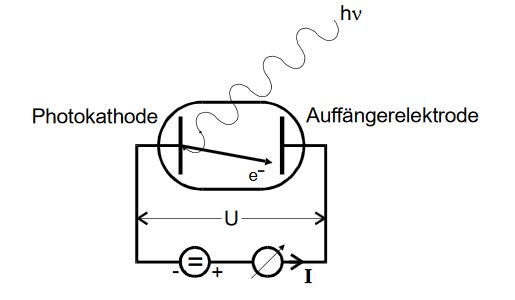
\includegraphics[width=0.6\textwidth]{aufbau.png}
 \caption{Darstellung und Schaltung einer Hochvakuumsdiode.\cite{sample}}
 \label{fig:aufbau}
 \end{figure}

\subsection{Sättigungsstrom}
Ausgehend von der Formel \eqref{eqn:näherung} und weiteren Betrachtungen ergibt sich
die Sättigungsstromdichte:
\begin{align}
j_\mathrm{s}(T)=4\pi\frac{e_\mathrm{0} m_\mathrm{0} k^2}{h^3} T^2 e^{\frac{-e_\mathrm{0}\Phi}{kT}} \label{eqn:st}.
\end{align}
Die Größen $m_\mathrm{0}$ und $h$ bschreiben die Elektronenmasse und das Planksche Wirkungsquantum.
Die Sättigungsstromdichte gibt die Anahl der austretenden Elektronen pro Zeit-und Flächeneinheit
in Abhängigkeit von der Temperatur wieder.

\subsection{Langmuir-Schottkysche Raumladungsdichte}
Bei der Messung des Anodenstroms zeigt sich eine Abhängigkeit von der Anodenspannung.
Erst bei einer hinreichend großen Anodenspannung wird der Strom unabhängig von der Spannung.
Dies hängt mit der zur Anode hin abnehmenden Raumladungsdichte zusammen, welche einen Einfluss
auf die Feldstärke zwischen Anode und Kathode hat. Die Feldlinien, ausgehend von der Anode, enden
an den Raumladungselektronen vor der Kathode. Der Diodenstrom fällt somit kleiner aus als erwartet.
Für den Zusammenhang von Anodenspannung und Anodenstrom im Raumladungsbereich wird die
Poissonsche Gleichung
\begin{align}
\Delta V =-\frac{1}{\epsilon_\mathrm{0}}\rho
\end{align}
herangezogen. $V$ beschreibt das Potential am Aufpunkt und $\epsilon_\mathrm{0}$ die Dielektrizitätskonstante.
Nach weiteren Rechnungen folgt daraus das Langmuir-Schottkysche Raumladungsgesetzt:
\begin{align}
j=\frac{4}{9}\epsilon_\mathrm{0}\sqrt{\frac{e_\mathrm{0}}{m_\mathrm{0}}}\frac{V^{\frac{3}{2}}}{a^2} .\label{eqn:LRS}
\end{align}
Stromdichte und Spannung sind nicht direkt proportional, wie es der Fall beim ohmschen Gesetzt ist, sondern
hier wächst $j$ mit $V^{\frac{3}{2}}$. Diese Gesetzmäßigkeit ist gültig im Raumladungsgebiet einer Hochvakuumdiode.
Wie sich das Potential $V$, die Feldstärke $E$ und die Raumladungsdichte $\rho$ im Raumladungsgebiet
verhalten, zeigt die Abbildung \ref{fig:verlauf}.
\begin{figure}
 \centering
 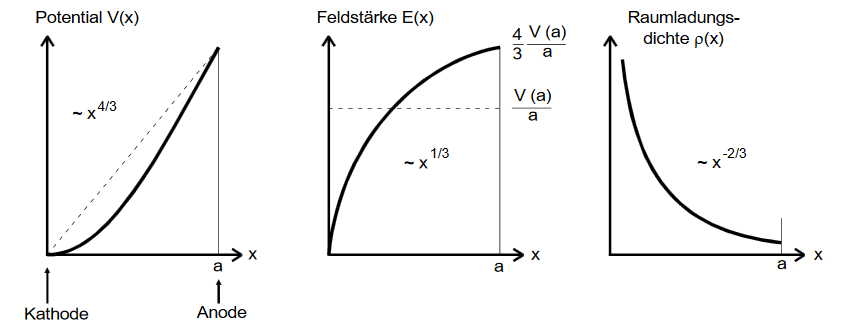
\includegraphics[width=0.5\textwidth]{verlauf.png}
 \caption{Ortsabhängigkeit von $V$, $E$ und $\rho$ im Raumladungsgebiet einer Hochvakuumsdiode.\cite{sample}}
 \label{fig:verlauf}
 \end{figure}
Die gesstrichelte Linie beim Potential zeigt zum Vergleich einen linearen Zusammenhang
und die gestrichelte Linie beim E-Feld veranschaulicht die Feldstärke ohne Raumladungselektronen.

\subsection{Anlaufstromgebiet}
Die Gleichung \eqref{eqn:LRS} besagt, dass bei $V=0$ auch $j=0$ gilt. Im Experiment zeigt sich jedoch,
dass ein geringer Anodenstrom beobachtet werden kann. Dieser Strom stammt von der Eigengeschwindigkeit
der Elektronen, die nach dem Austreten aus der Kathode noch einen Überschuss an Energie besitzen.
Diese Elektronen können gegen ein geringes Gegenfeld anlaufen, daher stammt die Bezeichnung Anlaufstrom.
Die Abbildung \ref{fig:pv} zeigt die Potentialverhältnisse zwischen Anode und Kathode im Bereich des Anlaufstromes.
\begin{figure}
 \centering
 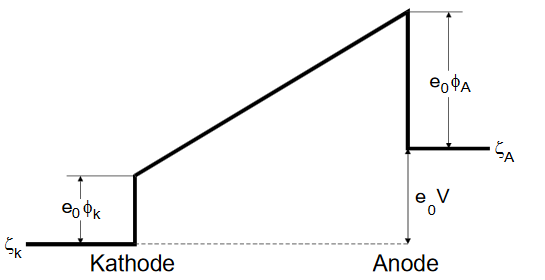
\includegraphics[width=0.5\textwidth]{pv.png}
 \caption{Potentialverhälnisse im Anlaufstromgebiet.\cite{sample}}
 \label{fig:pv}
 \end{figure}
Die die beiden sogenannten Fermi-Oberflächen unterscheiden sich um $e_\mathrm{0}V$, dies stammt von einem
äußeren Potential. Für die vom äußeren Potential $V$  abhängige Anlaufstromstärke gilt:
\begin{align}
j(V)=j_\mathrm{0}e^{\frac{-e_\mathrm{0}\Phi_\mathrm{A}+e_\mathrm{0}V}{kT}}=\mathrm{const}e^{-\frac{e_\mathrm{0}V}{kT}}\label{eqn:pot}.
\end{align}
\subsection{Kennlinie}
Um eine Kennlinie der Hochvakuumsdiode zu erhalten, wird der Anodenstrom gegen das äußere Potential
aufgetragen. Eine exemplarische Darstellung findet sich in Abbildung ?? wieder.
\begin{figure}
 \centering
 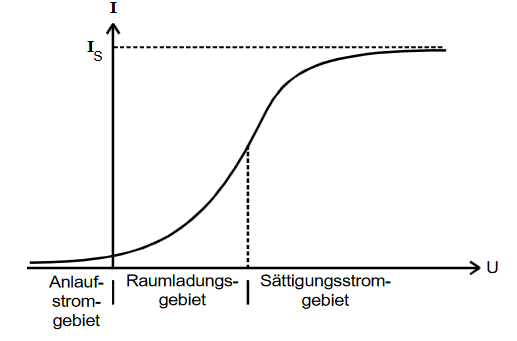
\includegraphics[width=0.5\textwidth]{kennlinie.png}
 \caption{Darstellung einer Kennlinie einer Hochvakuumsdiode.\cite{sample}}
 \label{fig:kennlinie}
 \end{figure}
Es lässt sich erkennen, dass im Anlaufstromgebiet ($V<0$) ein exponentieller zusammenhang
zwischen $I$ und $V$ besteht. Im Raumladungsgebiet besteht die $V^{\frac{3}{2}}$ Abhängigkeit, diese ist
allerdings nicht für beliebig hohe Anodenspannungen gültig. Der Anodenstrom strebt mit wachsendem $V$
einem Sättigungswert entgegen.
